\protect\hyperlink{main-nav}{≡} \protect\hyperlink{close-nav}{×}

\hypertarget{section-2.2-the-derivative}{%
\section{Section 2.2: The Derivative}\label{section-2.2-the-derivative}}

\hypertarget{instantaneous-velocity}{%
\subsection{Instantaneous Velocity}\label{instantaneous-velocity}}

Suppose we drop a tomato from the top of a 100 foot building and time
its fall.

\begin{figure}
\centering
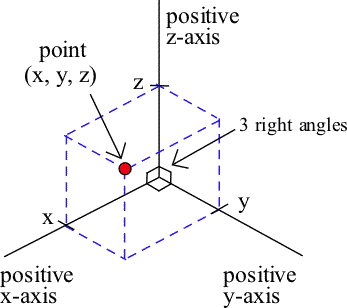
\includegraphics{images/image003.png}
\caption{}
\end{figure}

Some questions are easy to answer directly from the table:

\begin{enumerate}
\tightlist
\item
  How long did it take for the tomato n to drop 100 feet? (2.5 seconds)
\item
  How far did the tomato fall during the first second? (100 -- 84 = 16
  feet)
\item
  How far did the tomato fall during the last second? (64 -- 0 = 64
  feet)
\item
  How far did the tomato fall between \textbackslash{}(t
  =0.5\textbackslash{}) and \textbackslash{}(t = 1\textbackslash{})? (96
  -- 84 = 12 feet)
\end{enumerate}

Some questions require a little calculation:

\begin{enumerate}
\setcounter{enumi}{4}
\tightlist
\item
  What was the average velocity of the tomato during its fall?
  \textbackslash{}{[}\textbackslash{}text\{Average
  velocity\}=\textbackslash{}frac\{\textbackslash{}text\{distance
  fallen\}\}\{\textbackslash{}text\{total
  time\}\}=\textbackslash{}frac\{\textbackslash{}Delta\textbackslash{}text\{position\}\}\{\textbackslash{}Delta\textbackslash{}text\{time\}\}=\textbackslash{}frac\{-100
  \textbackslash{}text\{ ft\}\}\{2.5 \textbackslash{}text\{ s\}\}=-40
  \textbackslash{}text\{ ft/s\}\textbackslash{}{]}
\item
  What was the average velocity between \textbackslash{}(
  t=1\textbackslash{}) and \textbackslash{}(t=2\textbackslash{})
  seconds? \textbackslash{}{[}\textbackslash{}text\{Average
  velocity\}=\textbackslash{}frac\{\textbackslash{}Delta\textbackslash{}text\{position\}\}\{\textbackslash{}Delta\textbackslash{}text\{time\}\}=\textbackslash{}frac\{36\textbackslash{}text\{
  ft\}- 84\textbackslash{}text\{ ft\}\}\{2\textbackslash{}text\{ s\} -
  1\textbackslash{}text\{ s\}\}=\textbackslash{}frac\{-48
  \textbackslash{}text\{ ft\}\}\{1 \textbackslash{}text\{ s\}\}=-48
  \textbackslash{}text\{ ft/s\}\textbackslash{}{]}
\end{enumerate}

Some questions are more difficult:

\begin{enumerate}
\setcounter{enumi}{6}
\item
  How fast was the tomato falling 1 second after it was dropped?

  This question is significantly different from the previous two
  questions about average velocity. Here we want the
  \textbf{instantaneous velocity}, the velocity at an instant in time.
  Unfortunately the tomato is not equipped with a speedometer so we will
  have to give an approximate answer.

  One crude approximation of the instantaneous velocity after 1 second
  is simply the average velocity during the entire fall, -40 ft/s . But
  the tomato fell slowly at the beginning and rapidly near the end so
  the "-40 ft/s" estimate may or may not be a good answer.

  We can get a better approximation of the instantaneous velocity at
  \textbackslash{}(t=1\textbackslash{}) by calculating the average
  velocities over a short time interval near \textbackslash{}(t =
  1\textbackslash{}). The average velocity between \textbackslash{}(t =
  0.5\textbackslash{}) and \textbackslash{}(t = 1\textbackslash{}) is
  \textbackslash{}(\textbackslash{}dfrac\{-12\textbackslash{}text\{
  feet\}\}\{0.5\textbackslash{}text\{ s\}\} = -24\textbackslash{}text\{
  ft/s\}\textbackslash{}), and the average velocity between
  \textbackslash{}(t = 1\textbackslash{}) and \textbackslash{}(t =
  1.5\textbackslash{}) is
  \textbackslash{}(\textbackslash{}dfrac\{-20\textbackslash{}text\{
  feet\}\}\{0.5\textbackslash{}text\{ s\}\} = -40\textbackslash{}text\{
  ft/s\}\textbackslash{}) so we can be reasonably sure that the
  instantaneous velocity is between -24 ft/s and -40 ft/s.
\end{enumerate}

In general, the shorter the time interval over which we calculate the
average velocity, the better the average velocity will approximate the
instantaneous velocity. The average velocity over a time interval is
\textbackslash{}(
\textbackslash{}dfrac\{\textbackslash{}Delta\textbackslash{}text\{position\}\}\{\textbackslash{}Delta\textbackslash{}text\{time\}\}
\textbackslash{}), which is the slope of the \textbf{secant line}
through two points on the graph of height versus time. The instantaneous
velocity at a particular time and height is the slope of the
\textbf{tangent line} to the graph at the point given by that time and
height.

\begin{figure}
\centering
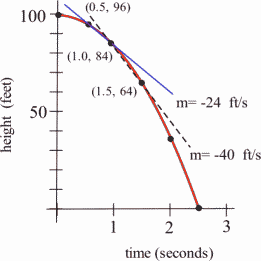
\includegraphics{images/image004.png}
\caption{}
\end{figure}

\hypertarget{average-vs-instantaneous-velocity}{%
\paragraph{Average vs Instantaneous
Velocity}\label{average-vs-instantaneous-velocity}}

\textbf{Average velocity} = \textbackslash{}(
\textbackslash{}dfrac\{\textbackslash{}Delta\textbackslash{}text\{position\}\}\{\textbackslash{}Delta\textbackslash{}text\{time\}\}
\textbackslash{}) = slope of the secant line through 2 points.

\textbf{Instantaneous velocity} = slope of the line tangent to the
graph.

\hypertarget{growing-bacteria}{%
\subsubsection{Growing Bacteria}\label{growing-bacteria}}

Suppose we set up a machine to count the number of bacteria growing on a
Petri plate. At first there are few bacteria so the population grows
slowly. Then there are more bacteria to divide so the population grows
more quickly. Later, there are more bacteria and less room and nutrients
available for the expanding population, so the population grows slowly
again. Finally, the bacteria have used up most of the nutrients, and the
population declines as bacteria die.

\begin{figure}
\centering
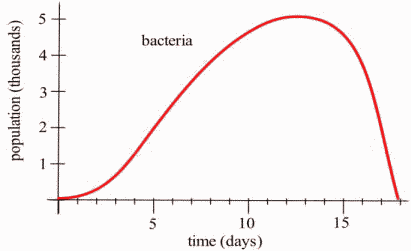
\includegraphics{images/image114.png}
\caption{}
\end{figure}

The population graph can be used to answer a number of questions.

\begin{enumerate}
\item
  What is the bacteria population at time \textbackslash{}(t =
  3\textbackslash{}) days?

  From the graph, at \textbackslash{}(t = 3\textbackslash{}), the
  population is about 0.5 thousand, or 500 bacteria.
\item
  What is the population increment from \textbackslash{}(t =
  3\textbackslash{}) to \textbackslash{}(t =10\textbackslash{}) days?

  At \textbackslash{}(t = 10\textbackslash{}), the population is about
  4.5 thousand, so the increment is about 4000 bacteria.
\item
  What is the \textbf{rate} of population growth from \textbackslash{}(t
  = 3\textbackslash{}) to \textbackslash{}(t = 10\textbackslash{}) days?

  The rate of growth from \textbackslash{}(t = 3\textbackslash{}) to
  \textbackslash{}(t = 10\textbackslash{}) is the average change in
  population during that time: \textbackslash{}{[}
  \textbackslash{}begin\{align*\} \textbackslash{}text\{average change
  in population \}=\& \textbackslash{}frac\{\textbackslash{}text\{change
  in population\}\}\{\textbackslash{}text\{change in
  time\}\}\textbackslash{}\textbackslash{} =\&
  \textbackslash{}frac\{\textbackslash{}Delta\textbackslash{}text\{population\}\}\{\textbackslash{}Delta\textbackslash{}text\{time\}\}
  \textbackslash{}\textbackslash{} =\&
  \textbackslash{}frac\{4000\textbackslash{}text\{
  bacteria\}\}\{7\textbackslash{}text\{ days\}\}
  \textbackslash{}\textbackslash{} \textbackslash{}approx\&
  570\textbackslash{}text\{ bacteria/day\}.
  \textbackslash{}end\{align*\} \textbackslash{}{]}

  This is the slope of the secant line through the two points (3, 500)
  and (10, 4500).
\item
  What is the \textbf{rate} of population growth on the third day, at
  \textbackslash{}(t = 3\textbackslash{}) ?

  This question is asking for the \textbf{instantaneous} rate of
  population change, the slope of the line which is \textbf{tangent} to
  the population curve at (3, 500). If we sketch a line approximately
  tangent to the curve at (3, 500) and pick two points near the ends of
  the tangent line segment , we can estimate that instantaneous rate of
  population growth is approximately 320 bacteria/day .

  \begin{figure}
  \centering
  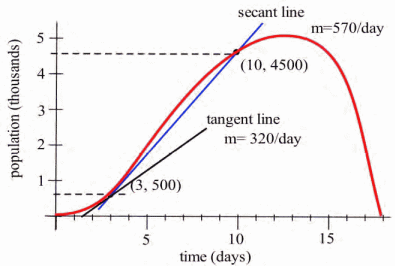
\includegraphics{images/image115.png}
  \caption{}
  \end{figure}
\end{enumerate}

\hypertarget{tangent-lines}{%
\subsection{Tangent Lines}\label{tangent-lines}}

\hypertarget{try-this}{%
\paragraph{Try this!}\label{try-this}}

The graph below is the graph of \textbackslash{}( y=f(x)
\textbackslash{}). We want to find the slope of the tangent line at the
point (1, 2).

\begin{figure}
\centering
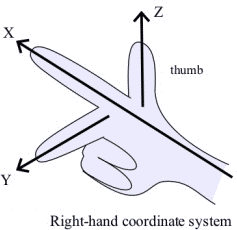
\includegraphics{images/image005.png}
\caption{}
\end{figure}

First, draw the secant line between (1, 2) and (2, −1) and compute its
slope.

Now draw the secant line between (1, 2) and (1.5, 1) and compute its
slope.

Compare the two lines you have drawn. Which would be a better
approximation of the tangent line to the curve at (1, 2)?

Now draw the secant line between (1, 2) and (1.3, 1.5) and compute its
slope. Is this line an even better approximation of the tangent line?

Now draw your best guess for the tangent line and measure its slope. Do
you see a pattern in the slopes?

You should have noticed that as the interval got smaller and smaller,
the secant line got closer to the tangent line and its slope got closer
to the slope of the tangent line. That's good news--we know how to find
the slope of a secant line.

In some applications, we need to know where the graph of a function
\textbackslash{}(f(x)\textbackslash{}) has horizontal tangent lines
(slopes = 0).

\hypertarget{example-1}{%
\paragraph{Example 1}\label{example-1}}

Below is the graph of \textbackslash{}(y = g(x)\textbackslash{}). At
what values of \textbackslash{}(x\textbackslash{}) does the graph of
\textbackslash{}(g(x)\textbackslash{}) have horizontal tangent lines?

\begin{figure}
\centering
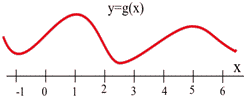
\includegraphics{images/image006.png}
\caption{}
\end{figure}

The tangent lines to the graph of \textbackslash{}(g(x)\textbackslash{})
are horizontal (slope = 0) when \textbackslash{}(x\textbackslash{}approx
-1, 1, 2.5, \textbackslash{}text\{ and \} 5\textbackslash{}).

To view this video please enable JavaScript, and consider upgrading to a
web browser that \href{http://videojs.com/html5-video-support/}{supports
HTML5 video}

Let's explore further this idea of finding the tangent slope based on
the secant slope.

\hypertarget{example-2}{%
\paragraph{Example 2}\label{example-2}}

Find the slope of the line \textbackslash{}(L\textbackslash{}) in the
graph below which is tangent to \textbackslash{}(f(x) =
x\^{}2\textbackslash{}) at the point (2,4).

We could estimate the slope of \textbackslash{}(L\textbackslash{}) from
the graph, but we won't. Instead, we will use the idea that secant lines
over tiny intervals approximate the tangent line.

\begin{figure}
\centering
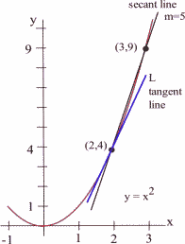
\includegraphics{images/image020.png}
\caption{}
\end{figure}

We can see that the line through (2,4) and (3,9) on the graph of
\textbackslash{}(f\textbackslash{}) is an approximation of the slope of
the tangent line, and we can calculate that slope exactly:
\textbackslash{}(m = \textbackslash{}frac\{\textbackslash{}Delta
y\}\{\textbackslash{}Delta x\} = \textbackslash{}frac\{9-4\}\{3-2\} =
5\textbackslash{}). But \textbackslash{}(m = 5\textbackslash{}) is only
an estimate of the slope of the tangent line and not a very good
estimate. It's too big. We can get a better estimate by picking a second
point on the graph of \textbackslash{}(f\textbackslash{}) which is
closer to (2,4) -- the point (2,4) is fixed and it must be one of the
points we use.

From the second figure, we can see that the slope of the line through
the points (2,4) and (2.5,6.25) is a better approximation of the slope
of the tangent line at (2,4): \textbackslash{}(m =
\textbackslash{}frac\{\textbackslash{}Delta y\}\{\textbackslash{}Delta
x\} = \textbackslash{}frac\{6.25 - 4\}\{2.5 - 2\} =
\textbackslash{}frac\{2.25\}\{0.5\} = 4.5 \textbackslash{}), a better
estimate, but still an approximation. We can continue picking points
closer and closer to (2,4) on the graph of
\textbackslash{}(f\textbackslash{}), and then calculating the slopes of
the lines through each of these points and the point (2,4):

\begin{longtable}[]{@{}lll@{}}
\caption{Points to the left of (2,4)}\tabularnewline
\toprule
\endhead
\textbackslash{}( x \textbackslash{}) & \textbackslash{}( y=x\^{}2
\textbackslash{}) & Slope of line through \textbackslash{}( (x,y)
\textbackslash{}) and (2,4).\tabularnewline
1.5 & 2.25 & 3.5\tabularnewline
1.9 & 3.61 & 3.9\tabularnewline
1.99 & 3.9601 & 3.99\tabularnewline
\bottomrule
\end{longtable}

\begin{longtable}[]{@{}lll@{}}
\caption{Points to the right of (2,4)}\tabularnewline
\toprule
\endhead
\textbackslash{}( x \textbackslash{}) & \textbackslash{}( y=x\^{}2
\textbackslash{}) & Slope of line through \textbackslash{}( (x,y)
\textbackslash{}) and (2,4).\tabularnewline
3 & 9 & 5\tabularnewline
2.5 & 6.25 & 4.5\tabularnewline
2.01 & 4.0401 & 4.01\tabularnewline
\bottomrule
\end{longtable}

The only thing special about the x--values we picked is that they are
numbers which are close, and very close, to \textbackslash{}(x =
2\textbackslash{}). Someone else might have picked other nearby values
for \textbackslash{}(x\textbackslash{}). As the points we pick get
closer and closer to the point (2,4) on the graph of \textbackslash{}( y
= x\^{}2\textbackslash{}), the slopes of the lines through the points
and (2,4) are better approximations of the slope of the tangent line,
and these slopes are getting closer and closer to 4.

We can bypass much of the calculating by not picking the points one at a
time: let's look at a general point near (2,4). Define \textbackslash{}(
x = 2 + h\textbackslash{}) so \textbackslash{}(h\textbackslash{}) is the
increment from 2 to \textbackslash{}(x\textbackslash{}). If
\textbackslash{}(h\textbackslash{}) is small, then \textbackslash{}(x =
2 + h\textbackslash{}) is close to 2 and the point
\textbackslash{}((2+h, f(2+h) ) = \textbackslash{}left(2+h,
(2+h)\^{}2\textbackslash{}right) \textbackslash{}) is close to (2,4).
The slope \textbackslash{}(m\textbackslash{}) of the line through the
points (2,4) and \textbackslash{}(\textbackslash{}left(2+h,
(2+h)\^{}2\textbackslash{}right)\textbackslash{}) is a good
approximation of the slope of the tangent line at the point (2,4):

\begin{figure}
\centering
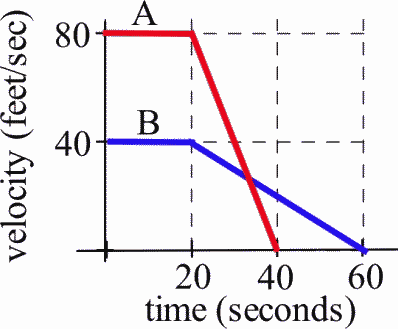
\includegraphics{images/image022.png}
\caption{\textbackslash{}(
m=\textbackslash{}dfrac\{(2+h)\^{}2-4\}\{(2+h)-2\}=\textbackslash{}dfrac\{\textbackslash{}left(4+4h+h\^{}2\textbackslash{}right)-4\}\{h\}=\textbackslash{}dfrac\{4h+h\^{}2\}\{h\}=\textbackslash{}dfrac\{h(4+h)\}\{h\}=4+h\textbackslash{})}
\end{figure}

The value \textbackslash{}( m = 4 + h \textbackslash{}) is the slope of
the secant line through the two points (2,4) and
\textbackslash{}(\textbackslash{}left( 2+h, (2+h)\^{}2
\textbackslash{}right)\textbackslash{}). As
\textbackslash{}(h\textbackslash{}) gets smaller and smaller, this slope
approaches the slope of the tangent line to the graph of
\textbackslash{}(f\textbackslash{}) at (2,4).

More formally, we could write:
\textbackslash{}{[}\textbackslash{}text\{Slope of the tangent line\} =
\textbackslash{}dfrac\{\textbackslash{}Delta y\}\{\textbackslash{}Delta
x\} = \textbackslash{}lim\textbackslash{}limits\_\{h\textbackslash{}to
0\} (4+h). \textbackslash{}{]}

We can easily evaluate this limit using direct substitution, finding
that as the interval \textbackslash{}(h\textbackslash{}) shrinks towards
0, the secant slope approaches the tangent slope, 4.

Try it for yourself using this applet:

\hypertarget{applet_container}{}

The tangent line problem and the instantaneous velocity problem are the
same problem. In each problem we wanted to know how rapidly something
was \textbf{changing at an instant in time}, and the answer turned out
to be finding the \textbf{slope of a tangent line}, which we
\emph{approximated} with the \textbf{slope of a secant line}. This idea
is the key to defining the slope of a curve.

To view this video please enable JavaScript, and consider upgrading to a
web browser that \href{http://videojs.com/html5-video-support/}{supports
HTML5 video}

\hypertarget{the-derivative}{%
\paragraph{The Derivative}\label{the-derivative}}

We can view the derivative in different ways. Here are a three of them:

\begin{itemize}
\tightlist
\item
  The derivative of a function \textbackslash{}(f\textbackslash{}) at a
  point (x, f(x)) is the instantaneous rate of change.
\item
  The derivative is the slope of the tangent line to the graph of
  \textbackslash{}(f\textbackslash{}) at the point \textbackslash{}((x,
  f(x))\textbackslash{}).
\item
  The derivative is the slope of the curve
  \textbackslash{}(f(x)\textbackslash{}) at the point
  \textbackslash{}((x, f(x))\textbackslash{}).
\end{itemize}

A function is called \textbf{differentiable} at \textbackslash{}((x,
f(x))\textbackslash{}) if its derivative exists at \textbackslash{}((x,
f(x))\textbackslash{}).

\hypertarget{notation-for-the-derivative}{%
\subparagraph{Notation for the
Derivative}\label{notation-for-the-derivative}}

The derivative of \textbackslash{}(y = f(x)\textbackslash{}) with
respect to \textbackslash{}(x\textbackslash{}) is written as
\textbackslash{}{[}f'(x)\textbackslash{}{]} (read aloud as
"\textbackslash{}(f\textbackslash{}) prime of
\textbackslash{}(x\textbackslash{})"), or
\textbackslash{}{[}y'\textbackslash{}{]} (read aloud as "why prime") or
\textbackslash{}{[}\textbackslash{}frac\{dy\}\{dx\}\textbackslash{}{]}
(read aloud as "dee why dee ex"), or
\textbackslash{}{[}\textbackslash{}frac\{df\}\{dx\}.\textbackslash{}{]}

The notation that resembles a fraction is called \textbf{Leibniz
notation}. It displays not only the name of the function
(\textbackslash{}(f\textbackslash{}) or
\textbackslash{}(y\textbackslash{})), but also the name of the variable
(in this case, \textbackslash{}(x\textbackslash{})). It looks like a
fraction because the derivative is a slope. In fact, this is simply
\textbackslash{}( \textbackslash{}frac\{\textbackslash{}Delta
y\}\{\textbackslash{}Delta x\} \textbackslash{}) written in Roman
letters instead of Greek letters.

\hypertarget{verb-forms}{%
\subparagraph{Verb Forms}\label{verb-forms}}

We \textbf{find the derivative} of a function, or \textbf{take the
derivative} of a function, or \textbf{differentiate} a function.

We use an adaptation of the \textbackslash{}(
\textbackslash{}frac\{df\}\{dx\} \textbackslash{}) notation to mean
"find the derivative of \textbackslash{}(f(x)\textbackslash{}):"
\textbackslash{}{[}\textbackslash{}frac\{d\}\{dx\}\textbackslash{}left{[}f(x)\textbackslash{}right{]}=\textbackslash{}frac\{df\}\{dx\}.\textbackslash{}{]}
{[}The book uses parentheses instead of brackets--both are acceptable
forms of the notation.{]}

\hypertarget{formal-algebraic-definition}{%
\subparagraph{Formal Algebraic
Definition}\label{formal-algebraic-definition}}

\textbackslash{}{[}f'(x)=\textbackslash{}lim\textbackslash{}limits\_\{h\textbackslash{}to
0\} \textbackslash{}dfrac\{f(x+h)-f(x)\}\{h\}\textbackslash{}{]}

\hypertarget{practical-definition}{%
\subparagraph{Practical Definition}\label{practical-definition}}

The derivative can be approximated by looking at an average rate of
change, or the slope of a secant line, over a very tiny interval. The
tinier the interval, the closer this is to the true instantaneous rate
of change, slope of the tangent line, or slope of the curve.

\hypertarget{looking-ahead}{%
\subparagraph{Looking Ahead}\label{looking-ahead}}

We will have methods for computing exact values of derivatives from
formulas soon. If the function is given to you as a table or graph, you
will still need to approximate this way.

To view this video please enable JavaScript, and consider upgrading to a
web browser that \href{http://videojs.com/html5-video-support/}{supports
HTML5 video}

This is the foundation for the rest of this chapter. It's remarkable
that such a simple idea (the slope of a tangent line) and such a simple
definition (for the derivative \textbackslash{}( f'(x)
\textbackslash{})) will lead to so many important ideas and
applications.

\hypertarget{example-3}{%
\paragraph{Example 3}\label{example-3}}

Find the slope of the tangent line to \textbackslash{}(
f(x)=\textbackslash{}frac\{1\}\{x\} \textbackslash{}) at
\textbackslash{}(x = 3\textbackslash{}).

The slope of the tangent line is the value of the derivative
\textbackslash{}(f'(3)\textbackslash{}). \textbackslash{}(
f(3)=\textbackslash{}frac\{1\}\{3\}\textbackslash{}) and
\textbackslash{}( f(3+h)=\textbackslash{}frac\{1\}\{3+h\}
\textbackslash{}), so, using the formal limit definition of the
derivative, \textbackslash{}{[}
f'(3)=\textbackslash{}lim\textbackslash{}limits\_\{h\textbackslash{}to
0\}\textbackslash{}frac\{f(3+h)-f(3)\}\{h\}=\textbackslash{}lim\textbackslash{}limits\_\{h\textbackslash{}to
0\}\textbackslash{}frac\{\textbackslash{}frac\{1\}\{3+h\}-\textbackslash{}frac\{1\}\{3\}\}\{h\}.
\textbackslash{}{]}

We can simplify by giving the fractions a common denominator:
\textbackslash{}{[} \textbackslash{}begin\{align*\}
\textbackslash{}lim\textbackslash{}limits\_\{h\textbackslash{}to
0\}\textbackslash{}frac\{\textbackslash{}frac\{1\}\{3+h\}-\textbackslash{}frac\{1\}\{3\}\}\{h\}=\&
\textbackslash{}lim\textbackslash{}limits\_\{h\textbackslash{}to
0\}\textbackslash{}frac\{\textbackslash{}frac\{1\}\{3+h\}\textbackslash{}cdot\textbackslash{}frac\{3\}\{3\}-\textbackslash{}frac\{1\}\{3\}\textbackslash{}cdot\textbackslash{}frac\{3+h\}\{3+h\}\}\{h\}
\textbackslash{}\textbackslash{} =\&
\textbackslash{}lim\textbackslash{}limits\_\{h\textbackslash{}to
0\}\textbackslash{}frac\{\textbackslash{}frac\{3\}\{9+3h\}-\textbackslash{}frac\{3+h\}\{9+3h\}\}\{h\}
\textbackslash{}\textbackslash{} =\&
\textbackslash{}lim\textbackslash{}limits\_\{h\textbackslash{}to
0\}\textbackslash{}frac\{\textbackslash{}frac\{3-(3+h)\}\{9+3h\}\}\{h\}
\textbackslash{}\textbackslash{} =\&
\textbackslash{}lim\textbackslash{}limits\_\{h\textbackslash{}to
0\}\textbackslash{}frac\{\textbackslash{}frac\{3-3-h\}\{9+3h\}\}\{h\}
\textbackslash{}\textbackslash{} =\&
\textbackslash{}lim\textbackslash{}limits\_\{h\textbackslash{}to
0\}\textbackslash{}frac\{\textbackslash{}frac\{-h\}\{9+3h\}\}\{h\}
\textbackslash{}\textbackslash{} =\&
\textbackslash{}lim\textbackslash{}limits\_\{h\textbackslash{}to
0\}\textbackslash{}frac\{-h\}\{9+3h\}\textbackslash{}cdot\textbackslash{}frac\{1\}\{h\}
\textbackslash{}\textbackslash{} =\&
\textbackslash{}lim\textbackslash{}limits\_\{h\textbackslash{}to
0\}\textbackslash{}frac\{-1\}\{9+3h\} \textbackslash{}\textbackslash{}
\textbackslash{}end\{align*\} \textbackslash{}{]} and the evaluate using
direct substitution:
\textbackslash{}{[}\textbackslash{}lim\textbackslash{}limits\_\{h\textbackslash{}to
0\}\textbackslash{}frac\{-1\}\{9+3h\}=\textbackslash{}frac\{-1\}\{9+3(0)\}=-\textbackslash{}frac\{1\}\{9\}.\textbackslash{}{]}

Thus, the slope of the tangent line to \textbackslash{}(
f(x)=\textbackslash{}frac\{1\}\{x\} \textbackslash{}) at
\textbackslash{}(x = 3\textbackslash{}) is \textbackslash{}(
-\textbackslash{}frac\{1\}\{9\} \textbackslash{}).

\hypertarget{the-derivative-as-a-function}{%
\subsection{The Derivative as a
Function}\label{the-derivative-as-a-function}}

We now know how to find (or at least approximate) the derivative of a
function for any \textbackslash{}(x\textbackslash{})-value; this means
we can think of the derivative as a function, too. The inputs are the
same \textbackslash{}(x\textbackslash{})'s; the output is the value of
the derivative at that \textbackslash{}(x\textbackslash{}) value.

\hypertarget{example-4}{%
\paragraph{Example 4}\label{example-4}}

Below is the graph of a function \textbackslash{}( y=f(x)
\textbackslash{}). We can use the information in the graph to fill in a
table showing values of \textbackslash{}( f'(x): \textbackslash{})

\begin{figure}
\centering
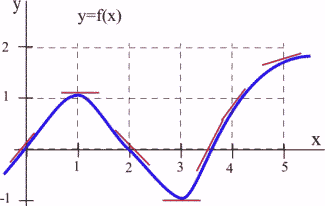
\includegraphics{images/image023.png}
\caption{}
\end{figure}

At various values of \textbackslash{}(x\textbackslash{}), draw your best
guess at the tangent line and measure its slope. You might have to
extend your lines so you can read some points. In general, your estimate
of the slope will be better if you choose points that are easy to read
and far away from each other. Here are estimates for a few values of
\textbackslash{}(x\textbackslash{}) (parts of the tangent lines used are
shown above in the graph):

\begin{longtable}[]{@{}lll@{}}
\toprule
\endhead
\textbackslash{}( x \textbackslash{}) & \textbackslash{}( y=f(x)
\textbackslash{}) & \textbackslash{}( f'(x)= \textbackslash{}) the
estimated \emph{slope} of the tangent line to the curve at the point
\textbackslash{}( (x,y) \textbackslash{}).\tabularnewline
0 & 0 & 1\tabularnewline
1 & 1 & 0\tabularnewline
2 & 0 & -1\tabularnewline
3 & -1 & 0\tabularnewline
3.5 & 0 & 2\tabularnewline
\bottomrule
\end{longtable}

We can estimate the values of \textbackslash{}(f'(x)\textbackslash{}) at
some non-integer values of \textbackslash{}(x\textbackslash{}), too:
\textbackslash{}(f'(0.5) \textbackslash{}approx 0.5\textbackslash{}) and
\textbackslash{}(f'(1.3) \textbackslash{}approx -0.3\textbackslash{}).

We can even think about entire intervals. For example, if
\textbackslash{}(0 \textbackslash{}lt x \textbackslash{}lt
1\textbackslash{}), then \textbackslash{}(f(x)\textbackslash{}) is
increasing, all the slopes are positive, and so
\textbackslash{}(f'(x)\textbackslash{}) is positive.

The values of \textbackslash{}(f'(x)\textbackslash{}) definitely depend
on the values of \textbackslash{}(x\textbackslash{}), and
\textbackslash{}(f'(x)\textbackslash{}) is a function of
\textbackslash{}(x\textbackslash{}). We can use the results in the table
to help sketch the graph of \textbackslash{}(f'(x)\textbackslash{}).

\begin{figure}
\centering
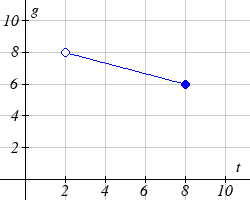
\includegraphics{images/image024.png}
\caption{}
\end{figure}

To view this video please enable JavaScript, and consider upgrading to a
web browser that \href{http://videojs.com/html5-video-support/}{supports
HTML5 video}

\hypertarget{example-5}{%
\paragraph{Example 5}\label{example-5}}

Shown is the graph of the height \textbackslash{}(h(t)\textbackslash{})
of a rocket at time \textbackslash{}(t\textbackslash{}).

\begin{figure}
\centering
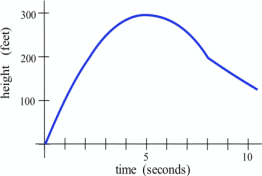
\includegraphics{images/image025.png}
\caption{}
\end{figure}

Sketch the graph of the \textbf{velocity} of the rocket at time
\textbackslash{}(t\textbackslash{}). (Velocity is the
\textbf{derivative} of the height function, so it is the \textbf{slope
of the tangent} to the graph of position or height.)

We can estimate the slope of the function at several points. The lower
graph below shows the velocity of the rocket. This is
\textbackslash{}(v(t) = h'(t)\textbackslash{}).

\begin{figure}
\centering
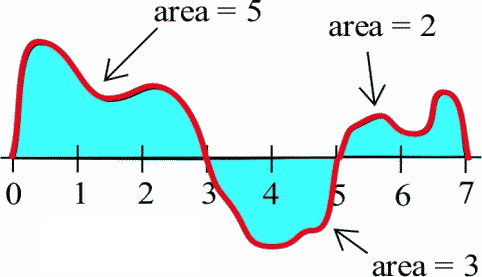
\includegraphics{images/image026.png}
\caption{}
\end{figure}

We can also find derivative functions algebraically using limits.

\hypertarget{example-6}{%
\paragraph{Example 6}\label{example-6}}

Find \textbackslash{}(
\textbackslash{}frac\{d\}\{dx\}\textbackslash{}left( 2x\^{}2-4x-1
\textbackslash{}right) \textbackslash{}).

Setting up the derivative using a limit, \textbackslash{}{[}
f'(x)=\textbackslash{}lim\textbackslash{}limits\_\{h\textbackslash{}to
0\}\textbackslash{}frac\{f(x+h)-f(x)\}\{h\}.\textbackslash{}{]}

We will start by simplifying \textbackslash{}( f(x+h) \textbackslash{})
by expanding: \textbackslash{}{[} \textbackslash{}begin\{align*\}
f(x+h)=\& 2(x+h)\^{}2-4(x+h)-1 \textbackslash{}\textbackslash{} =\&
2(x\^{}2+2xh+h\^{}2)-4(x+h)-1 \textbackslash{}\textbackslash{} =\&
2x\^{}2+4xh+2h\^{}2-4x-4h-1 \textbackslash{}end\{align*\}
\textbackslash{}{]}

Now finding the limit: \textbackslash{}{[}
\textbackslash{}begin\{align*\} f'(x)=\&
\textbackslash{}lim\textbackslash{}limits\_\{h\textbackslash{}to
0\}\textbackslash{}frac\{f(x+h)-f(x)\}\{h\}
\textbackslash{}\textbackslash{} =\&
\textbackslash{}lim\textbackslash{}limits\_\{h\textbackslash{}to 0\}
\textbackslash{}frac\{(2x\^{}2+4xh+2h\^{}2-4x-4h-1)-(2x\^{}2-4x-1)\}\{h\}
\textbackslash{}\textbackslash{} =\&
\textbackslash{}lim\textbackslash{}limits\_\{h\textbackslash{}to 0\}
\textbackslash{}frac\{2x\^{}2+4xh+2h\^{}2-4x-4h-1-2x\^{}2+4x+1\}\{h\}
\textbackslash{}qquad \textbackslash{}text\{(Substitute in the
formulas.)\} \textbackslash{}\textbackslash{} =\&
\textbackslash{}lim\textbackslash{}limits\_\{h\textbackslash{}to 0\}
\textbackslash{}frac\{4xh+2h\^{}2-4h\}\{h\} \textbackslash{}qquad
\textbackslash{}text\{(Now simplify.)\}\textbackslash{}\textbackslash{}
=\& \textbackslash{}lim\textbackslash{}limits\_\{h\textbackslash{}to 0\}
\textbackslash{}frac\{h(4x+2h-4)\}\{h\} \textbackslash{}qquad
\textbackslash{}text\{(Factor out the \textbackslash{}( h
\textbackslash{}), then cancel.)\} \textbackslash{}\textbackslash{} =\&
\textbackslash{}lim\textbackslash{}limits\_\{h\textbackslash{}to 0\}
(4x+2h-4) \textbackslash{}end\{align*\} \textbackslash{}{]} We can find
the limit of this expression by direct substitution: \textbackslash{}{[}
f'(x)=\textbackslash{}lim\textbackslash{}limits\_\{h\textbackslash{}to
0\} (4x+2h-4)=4x-4\textbackslash{}{]}

Notice that the derivative depends on
\textbackslash{}(x\textbackslash{}), and that this formula will tell us
the slope of the tangent line to \textbackslash{}(f\textbackslash{}) at
any value \textbackslash{}(x\textbackslash{}). For example, if we wanted
to know the tangent slope of \textbackslash{}(f\textbackslash{}) at
\textbackslash{}(x = 3\textbackslash{}), we would simply evaluate:
\textbackslash{}( f'(3)=4(3)-4=8 \textbackslash{}).

A formula for the derivative function is very powerful, but as you can
see, calculating the derivative using the limit definition is
\textbf{very} time consuming. In the next section, we will identify some
patterns that will allow us to start building a set of rules for finding
derivatives without needing the limit definition.

\hypertarget{interpreting-the-derivative}{%
\subsection{Interpreting the
Derivative}\label{interpreting-the-derivative}}

So far we have emphasized the derivative as the slope of the line
tangent to a graph. That interpretation is very visual and useful when
examining the graph of a function, and we will continue to use it.
Derivatives, however, are used in a wide variety of fields and
applications, and some of these fields use other interpretations. The
following are a few interpretations of the derivative that are commonly
used.

\hypertarget{general}{%
\paragraph{General}\label{general}}

Rate of Change: \textbackslash{}(f '(x)\textbackslash{}) is the
\textbf{rate of change} of the function at
\textbackslash{}(x\textbackslash{}). If the units for
\textbackslash{}(x\textbackslash{}) are years and the units for
\textbackslash{}(f(x)\textbackslash{}) are people, then the units for
\textbackslash{}( \textbackslash{}frac\{df\}\{dx\} \textbackslash{}) are
\textbackslash{}(\textbackslash{}frac\{\textbackslash{}text\{people\}\}\{\textbackslash{}text\{year\}\}\textbackslash{}),
a rate of change in population.

\hypertarget{graphical}{%
\paragraph{Graphical}\label{graphical}}

Slope: \textbackslash{}(f '(x)\textbackslash{}) is the \textbf{slope of
the line tangent to the graph of \textbackslash{}(f\textbackslash{}) at
the point \textbackslash{}(( x, f(x) )\textbackslash{})}.

\hypertarget{physical}{%
\paragraph{Physical}\label{physical}}

Velocity: If \textbackslash{}(f(x)\textbackslash{}) is the position of
an object at time \textbackslash{}(x\textbackslash{}), then
\textbackslash{}(f '(x)\textbackslash{}) is the \textbf{velocity} of the
object at time \textbackslash{}(x\textbackslash{}). If the units for
\textbackslash{}(x\textbackslash{}) are hours and
\textbackslash{}(f(x)\textbackslash{}) is distance measured in miles,
then the units for \textbackslash{}(f '(x) =
\textbackslash{}frac\{df\}\{dx\}\textbackslash{}) are \textbackslash{}(
\textbackslash{}frac\{\textbackslash{}text\{miles\}\}\{\textbackslash{}text\{hour\}\}
\textbackslash{}), miles per hour, which is a measure of velocity.

Acceleration: If \textbackslash{}(f(x)\textbackslash{}) is the velocity
of an object at time \textbackslash{}(x\textbackslash{}), then
\textbackslash{}(f '(x)\textbackslash{}) is the \textbf{acceleration} of
the object at time \textbackslash{}(x\textbackslash{}). If the units are
for \textbackslash{}(x\textbackslash{}) are hours and
\textbackslash{}(f(x)\textbackslash{}) has the units \textbackslash{}(
\textbackslash{}frac\{\textbackslash{}text\{miles\}\}\{\textbackslash{}text\{hour\}\}
\textbackslash{}), then the units for the acceleration
\textbackslash{}(f '(x) =
\textbackslash{}frac\{df\}\{dx\}\textbackslash{}) are \textbackslash{}(
\textbackslash{}frac\{\textbackslash{}text\{miles/hour\}\}\{\textbackslash{}text\{hour\}\}
=\textbackslash{}frac\{\textbackslash{}text\{miles\}\}\{\textbackslash{}text\{hour\}\^{}2\}
\textbackslash{}), miles per hour per hour.

\hypertarget{business}{%
\paragraph{Business}\label{business}}

Marginal Cost, Marginal Revenue, and Marginal Profit: We'll explore
these terms in more depth later in the section. Basically, the marginal
cost is approximately the \emph{additional} cost of making one more
object once we have already made \textbackslash{}(x\textbackslash{})
objects. If the units for \textbackslash{}(x\textbackslash{}) are
bicycles and the units for \textbackslash{}(f(x)\textbackslash{}) are
dollars, then the units for \textbackslash{}(f '(x) =
\textbackslash{}frac\{df\}\{dx\}\textbackslash{}) are \textbackslash{}(
\textbackslash{}frac\{\textbackslash{}text\{dollars\}\}\{\textbackslash{}text\{
bicycle\}\} \textbackslash{}), the cost per bicycle.

In business contexts, the word "\textbf{marginal}" usually means the
derivative or rate of change of some quantity.

One of the strengths of calculus is that it provides a unity and economy
of ideas among diverse applications. The vocabulary and problems may be
different, but the ideas and even the notations of calculus are still
useful.

\hypertarget{example-7}{%
\paragraph{Example 7}\label{example-7}}

Suppose the demand curve for widgets was given by \textbackslash{}(
D(p)=\textbackslash{}frac\{1\}\{p\} \textbackslash{}), where
\textbackslash{}(D\textbackslash{}) is the quantity of widgets, in
thousands, at a price of \textbackslash{}(p\textbackslash{}) dollars.
Interpret the derivative of \textbackslash{}(D\textbackslash{}) at
\textbackslash{}(p = \textbackslash{})\$3.

Note that we calculated \textbackslash{}( D'(3) \textbackslash{})
earlier to be \textbackslash{}(
D'(3)=-\textbackslash{}frac\{1\}\{9\}\textbackslash{}approx -0.111
\textbackslash{}).

Since \textbackslash{}(D\textbackslash{}) has units ``thousands of
widgets'' and the units for \textbackslash{}(p\textbackslash{}) is
dollars of price, the units for \textbackslash{}(D'\textbackslash{})
will be \textbackslash{}(
\textbackslash{}frac\{\textbackslash{}text\{thousands of
widgets\}\}\{\textbackslash{}text\{dollar of price\}\}
\textbackslash{}). In other words, it shows how the demand will change
as the price increases.

Specifically, \textbackslash{}( D'(3)\textbackslash{}approx -0.111
\textbackslash{}) tells us that when the price is \$3, the demand will
\emph{decrease} by about 0.111 thousand items for every dollar the price
increases.

(Note: The screen shots in the following video are from an earlier
version of the book, so some of the section numbers or titles may not
look the same. However, much of the content is the same, and the
comments still apply.)

To view this video please enable JavaScript, and consider upgrading to a
web browser that \href{http://videojs.com/html5-video-support/}{supports
HTML5 video}

\begin{longtable}[]{@{}ll@{}}
\toprule
\endhead
\href{section2-1.php}{← Previous Section} & \href{section2-3.php}{Next
Section →}\tabularnewline
\bottomrule
\end{longtable}
